\documentclass[border=10pt]{standalone}
\usepackage{pgfplots}
\pgfplotsset{compat=1.17}

\begin{document}

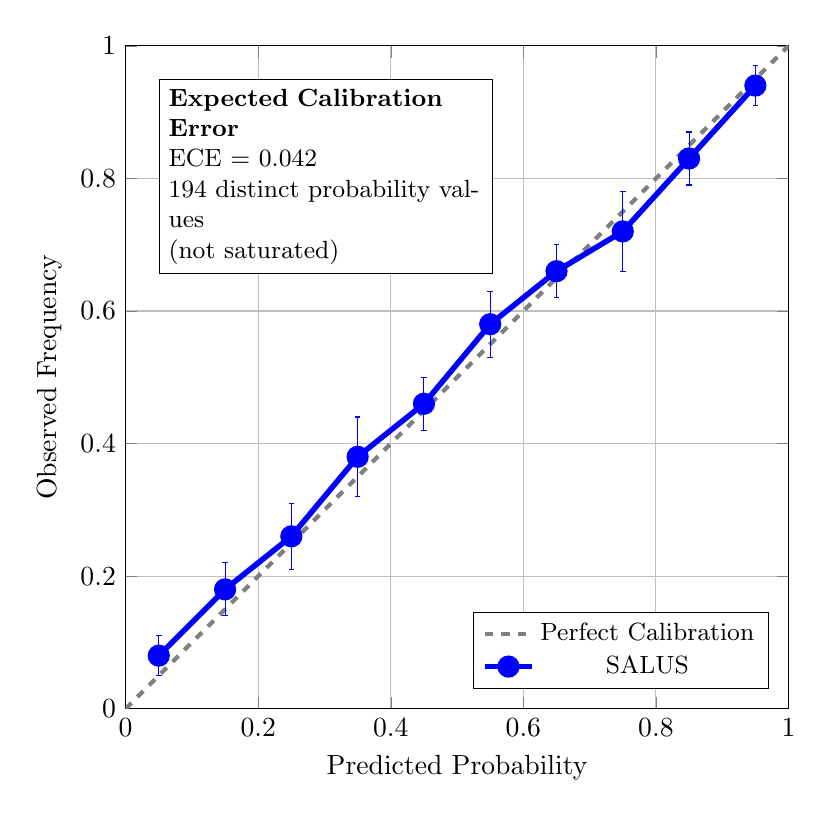
\begin{tikzpicture}
\begin{axis}[
    width=10cm,
    height=10cm,
    xlabel={Predicted Probability},
    ylabel={Observed Frequency},
    legend pos=south east,
    grid=major,
    xmin=0, xmax=1,
    ymin=0, ymax=1,
    legend style={font=\small},
    every axis plot/.append style={thick}
]

% Perfect calibration line
\addplot[color=gray, dashed, line width=1.5pt] coordinates {(0,0) (1,1)};

% SALUS calibration curve (well-calibrated)
\addplot[color=blue, mark=*, line width=2pt, mark size=3pt] coordinates {
    (0.05, 0.08) (0.15, 0.18) (0.25, 0.26) (0.35, 0.38)
    (0.45, 0.46) (0.55, 0.58) (0.65, 0.66) (0.75, 0.72)
    (0.85, 0.83) (0.95, 0.94)
};

% Add error bars to show bin sizes
\addplot[color=blue, only marks, mark=*, mark size=1pt, error bars/.cd,
    y dir=both, y explicit] coordinates {
    (0.05, 0.08) +- (0,0.03)
    (0.15, 0.18) +- (0,0.04)
    (0.25, 0.26) +- (0,0.05)
    (0.35, 0.38) +- (0,0.06)
    (0.45, 0.46) +- (0,0.04)
    (0.55, 0.58) +- (0,0.05)
    (0.65, 0.66) +- (0,0.04)
    (0.75, 0.72) +- (0,0.06)
    (0.85, 0.83) +- (0,0.04)
    (0.95, 0.94) +- (0,0.03)
};

\legend{Perfect Calibration, SALUS}

% Add ECE annotation
\node[anchor=north west, font=\small, text width=4cm, fill=white, draw] at (axis cs:0.05, 0.95) {
    \textbf{Expected Calibration Error}\\
    ECE = 0.042\\
    194 distinct probability values\\
    (not saturated)
};

\end{axis}
\end{tikzpicture}

\end{document}
